\documentclass{homework}
% \usepackage{graphicx} % Required for inserting images
\usepackage{amsmath}
\usepackage{gensymb}
\usepackage{subfig}
\usepackage{float}

\usepackage{algorithm}
\usepackage{algpseudocode}

\class{APPM 5560}
\title{Homework 5}
\author{Sean Jennings}
\date{March 7, 2024}

\begin{document}
\maketitle

\section{Problem 1}
For simplicity, assume that the markov chain is finite. Then,
the markov chain can be described by the probability transition
matrix $p\in\R^{n\times n}$. Since $\pi_1$ and $\pi_2$ are 
stationary distributions, we have
\begin{equation*}
    \pi_1 = \pi_1 p \qquad \pi_2 = \pi_2 p.
\end{equation*}
We first check the stationarity condition:
\begin{align*}
    \pi_3 p &= [\lambda \pi_1 + (1 - \lambda) \pi_2] p \\
        &= \lambda ( \pi_1 p ) + (1 - \lambda) (\pi_2 p) \\
        &= \lambda \pi_1 + (1 - \lambda) \pi_2 \\
        &= \pi_3.
\end{align*}
Thus, $\pi_3 p = \pi_3$ is satisfied.

Next, we check that each entry of $\pi_3$ is a valid probability
(i.e. $0 \leq \pi_3(i) \leq 1$ for all $i$). Each entry of $\pi_1$
and $\pi_2$ has
\begin{equation*}
    0 \leq \pi_1(i) \leq 1 \qquad
    0 \leq \pi_2(i) \leq 1
\end{equation*}
so by multiplying by $\lambda$ and $1 - \lambda$, respectively, we then have:
\begin{equation*}
    0 \leq \lambda \pi_1(i) \leq \lambda \qquad
    0 \leq (1 - \lambda) \pi_2(i) \leq 1 - \lambda.
\end{equation*}
(Note that these inequality hold since the bounds $0 \leq \lambda \leq 1$
imply that both $\lambda$ and $1 - \lambda$ are non-negative.)

Summing these equations yields:
\begin{equation*}
    0 \leq \lambda \pi_1(i) + (1 - \lambda) \pi_2(i) \leq \lambda + (1 - \lambda) = 1.
\end{equation*}
So we have $0\leq \pi_3(i) \leq 1$ for each $i$.

Finally, we see that since $\pi_1$ and $\pi_2$ satisfy the normalization property,
$\pi_3$ does as well:
\begin{align*}
    \sum_i \pi_3(i) &= \sum_i \lambda \pi_1(i) + (1 - \lambda) \pi_2(i) \\
        &= \lambda \sum_i \pi_1(i) + (1 - \lambda) \sum_i \pi_2(i) \\
        &= \lambda + (1 - \lambda) = 1
\end{align*}

When the state space is infinite, right multiplication by the probability transition
matrix can be replaced by a generic linear transformation between
infinite-dimensional vector spaces and the same result follows from the linearity
of that transformation.


\section{Problem 2}
\begin{letterenum}
\item Let $N$ be the number of columns of square matrix $p$.
Since the sum of each row of $p$ is 1, it follows that
the $i$-th entry of $p \one$ is given by:
\begin{align*}
    (p \one)_i = \sum_{j=1}^N p(i,j) 1 = \sum_{j=1}^N p(i,j) = 1
\end{align*}
where $\one\in\R^N$ is the vector of all ones. Therefore, $p \one = (1) \one$
and $\one$ is an eigenvector of $p$ with eigenvalue 1.

\item By the Gershgorin circle theorem, each eigenvalue of $p$ lies within
\begin{equation*}
    D(p(i, i), R_i) \subseteq \C,
\end{equation*}
the disc in the complex plane centered at $p(i, i)$ with radius $R_i$ given
by:
\begin{equation*}
    R_i = \sum_{j\neq i} |p(i, j)| = \sum_{j \neq i} p(i, j)
\end{equation*}
for some $i$.

But the maximum magnitude that $\lambda \in D(p(i, i), R_i)$ can take
within a given disk is $|p(i, i)| + R_i$ (i.e. when it lies on the edge of the disc
away from the origin). Thus, each eigenvalue $\lambda$ of matrix $p$
is upper bounded by the maximum magnitude across all discs is:
\begin{align*}
    |\lambda| &\leq \max_i \{|p(i, i)| + R_i\} \\
        &= \max_i \{p(i, i) + \sum_{j\neq i} p(i, j)\} \\
        &= \max_i \{\sum_{j=1}^{N} p(i, j)\} \\
        &= \max_i \{1 \} = 1.
\end{align*}

\section{Problem 3}
Since $A$ is a doubly stochastic matrix the sum of each row $i$ is
\begin{equation*}
    \sum_{j=1}^N A_{ij} = 1
\end{equation*}
(for each $i$), the sum of each column $j$ is
\begin{equation*}
    \sum_{i=1}^N A_{ij} = 1
\end{equation*}
(for each $j$), and likewise for $B$.

To see that $AB$ is doubly stochastic, we verify that $AB$ satisfies the
same properties. Using the definition of matrix multiplication and the
distributive property, we have the row sum of the $i$-th
column of $AB$ is:
\begin{align*}
    \sum_{j=1}^N (AB)_{ij} &= \sum_{j=1}^{N} \sum_{k=1}^N A_{ik} B_{kj} \\
        &= \sum_{k=1}^{N} \sum_{j=1}^N B_{kj} A_{ik} \\
        &= \sum_{k=1}^{N} \biggl(\sum_{j=1}^N B_{kj} \biggr) A_{ik} \\
        &= \sum_{k=1}^{N} A_{ik} = 1.
\end{align*}
Similarly, the sum of column $j$ is:
\begin{align*}
    \sum_{i=1}^N (AB)_{ij} &= \sum_{i=1}^N \sum_{k=1}^N A_{ik} B_{kj} \\
        &= \sum_{k=1}^N \biggl(\sum_{i=1}^N A_{ik} \biggr) B_{kj} \\
        &= \sum_{k=1}^N B_{kj} = 1.
\end{align*}
So the sum of each row and column of $AB$ equals 1 and $AB$ is also doubly
stochastic.
\end{letterenum}

\section{Problem 4}

Pseudocode to sample a discrete variable from a given initial distribution $\mu$
is given below
\begin{algorithmic}
    \Function{sampleDiscrete}{$\mu$}
        \State $\pi \gets $ reverse(argsort($\mu$))
        \Comment Permutation of indices in descending order
        \State \Comment This result should be cached to avoid excess
        \State \Comment computation on each simulation step below.

        \State $u \sim$ Uniform(0, 1) 
        \State $N \gets$ length($\mu$)
        \State cumsum $\gets 0$
        \For {$i \gets 1 $ {\bf to} $N$}
            \State cumsum $\gets$ cumsum + $\mu(\pi(i))$
            \If {u $\leq$ cumsum}
                \State \Return $\pi(i)$
            \EndIf
        \EndFor
    \EndFunction
\end{algorithmic}
Using this primitive, we simulate a general Markov chain with initial distribution
$\mu0$ and probability matrix $p$ for $n$ steps by sampling from the row of the
$p$ corresponding to the previous state:
\begin{algorithmic}
    \Function{SimulateMarkov}{$\mu0, p, n$}
        \State $X \gets $Array($n+1$)
        \Comment 0-indexed array of length $(n+1)$ containing
        \State \Comment simulation results $[X_0, X_1, \dots, X_n]$
        \State $X[0] = $sampleDiscrete($\mu0$)
        \For {$n \gets 1$ {\bf to} $N$}
            \State $X[n] = $sampleDiscrete$(p[X[n-1]])$
            \Comment $p[i]$ is the $i$-th row of the probability transition matrix
        \EndFor
        \State \Return X
    \EndFunction
\end{algorithmic}


\section{Problem 5}

\begin{letterenum}
\item By detailed balance, we have:
\begin{align*}
    \pi(k) &= \frac{\prod_{n=1}^{k-1} p_n}{\prod_{n=2}^k q_n} \pi(1) \\
        &= \frac{\prod_{n=1}^{k-1} \beta e^{\alpha n}}{\prod_{n=2}^k b e^{a(n-1)}} \pi(1) \\
        &= \biggl(\frac{\beta}{b}\biggr)^{k-1} \exp\biggl(
            \sum_{n=1}^{k-1} \alpha n - \sum_{n=2}^k a(n-1)
        \biggr) \pi(1)
\end{align*}

The summation in the exponent can be simplied as follows:
\begin{align*}
    \sum_{n=1}^{k-1} \alpha n - \sum_{m=2}^{k} a(m-1) 
        &= \sum_{n=1}^{k-1} \alpha n - \sum_{n=1}^{k-1} an \\
        &= (\alpha - a) \sum_{n=1}^{k-1} n \\
        &= (\alpha - a) \biggl(\frac{k(k-1)}{2}\biggr)
\end{align*}
And we can simplify the expression for $\pi(k)$ further to:
\begin{align*}
    \pi(k) &= \biggl[
        \biggl(\frac{\beta}{b}\biggr)^{k-1}
        e^{1/2 (\alpha - a)k(k-1)}
    \biggr] \pi(1) \\
    &= \biggl(
        \frac{\beta e^{1/2 (\alpha - a)k}}{b}
    \biggr)^{k-1} \pi(1)
\end{align*}

\item Code for numerically computing eigenvector with eigenvalue 1
is shown below.  By this method, we find the stationary distribution
is:

    
\begin{equation*}
    \pi = \mat{
            1.019\times 10^{-4} \\ 1.244\times 10^{-4} \\ 1.857\times 10^{-4}
            \\ 3.383\times 10^{-4} \\ 7.529\times 10^{-4} \\
            2.047\times 10^{-3} \\ 6.795\times 10^{-3}
            \\ 2.755\times 10^{-2} \\ 0.1365 \\ 0.8256
            }^T
\end{equation*}

\item We implement the pseudocode from problem 4 to simulate the markov chain
with the given parameters
\begin{align*}
    \beta = 0.001 & \qquad b=0.001 \\
    \alpha = 0.4 &\qquad a = 0.2
\end{align*}

Figure \ref{fig:sim-histogram} shows a histogram of the fraction of time
spent in the different states. Since the states on the left of the plot
are visited infrequently, we scale the y-axis logarithmically.


\begin{center}
    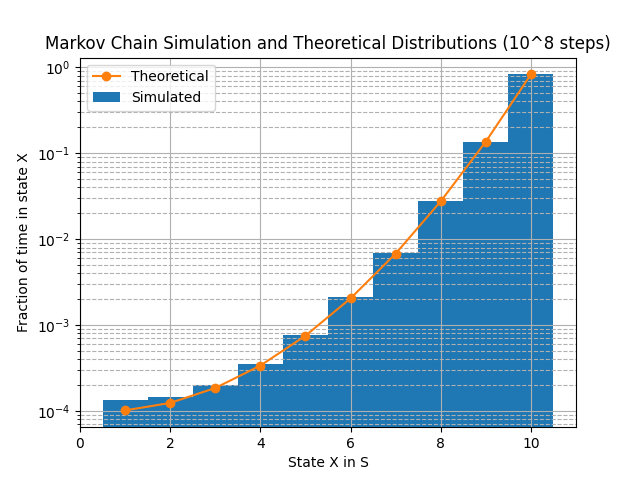
\includegraphics[width=0.8\linewidth]{Images/simulation.png}
    \captionof{figure}{Histogram of simulated Markov chain}
    \label{fig:sim-histogram}
\end{center}

\item The theoretical distributions and simulated distribution agree
very closely for the most probable states on the right of the chain.

Further left on the chain (e.g. states 1-3) there is a high variance in the amount
of time spent in those states (compared to the overall magnitude). Since these
states occur infrequently, the simulation can randomly stay in one particular
state a bit longer or shorter than the expected value. Just a few extra simulation
steps has an outsized impact because the expected number of simulation steps
spent in those states is so small to begin with. Conversely, it is easy for
the simulation to skip infrequent states entirely resulting in an underestimation
of the stationary distribution.

Emperically, the fraction of time spent in infrequent states begins to
converge to the stationary distribution after a large number of simulation steps.
The histogram shown in Figure \ref{fig:sim-histogram} was run for
$10^8$ steps and we begin to see convergence to the theoretical distribution
for all states.

\end{letterenum}

\section{Problem 6}

Since all chains are irreducible, the period is equal for each state in the chain.
The chain is aperiodic when that period equals 1. To determine the period for each 
example we select a particular state and search exhaustively for cycles (multi-step
paths which return the chain to the original state) and then find the GCF of the
path length of each cycle.

To determine the stationary distribution, we write down the probability transition
matrix and use the eigenvector-based numerical routine developed in Problem 5b
to avoid solving the systems of linear equations by hand.

\begin{letterenum}
\item Starting from state 2, there are two cycles:
\begin{enumerate}
    \item $2 \to 3 \to 1 \to 2$ (length 3), and
    \item $2 \to 1 \to 2$ (length 2)
\end{enumerate}
Thus, the period is GCF$\{2, 3, \dots\} = 1$ and the chain is aperiodic.

From the probability matrix
\begin{equation*}
    p = \mat{
        0 & 1 & 0 \\
        1/2 & 0 & 1/2 \\
        1 & 0 & 0
    }
\end{equation*}
we have stationary distribution
\begin{equation*}
    \pi = \mat{2/5 & 2/5 & 1/5}
\end{equation*}

\item From state 2, there are two cycles:
\begin{enumerate}
    \item $1 \to 2 \to 1$ (length 2)
    \item $1 \to 2 \to 3 \to 1$ (length 4)
\end{enumerate}
So the chain is periodic with period 2. 

Probability matrix
\begin{equation*}
    p = \mat{
        0 & 1 & 0 & 0 \\
        1/2 & 0 & 1/2 & 0 \\
        0 & 0 & 0 & 1 \\
        1 & 0 & 0 & 0
    }
\end{equation*}
gives stationary distribution:
\begin{equation*}
    \pi = \mat{1/3 & 1/3 & 1/6 & 1/6}
\end{equation*}

\item Cycles:
\begin{enumerate}
    \item $2 \to 4 \to 1 \to 2$ (length 3)
    \item $2 \to 3\to 4 \to 1 \to 2$ (length 4)
\end{enumerate}
The period (GCF of $\{3, 4, \dots\}$) is 1, so the chain is aperoidic.

Probability matrix
\begin{equation*}
    p = \mat{
        0 & 1 & 0 & 0 \\
        0 & 0 & 1/2 & 1/2 \\
        0 & 0 & 0 & 1 \\
        1 & 0 & 0 & 0
    }
\end{equation*}
gives stationary distribution:
\begin{equation*}
    \pi = \mat{2/7 & 2/7 & 1/7 & 2/7}
\end{equation*}

\item Cycles from state 2:
\begin{enumerate}
    \item $2 \to 5 \to 2$ (length 2),
    \item $2 \to 3 \to 4\to 5 \to 2$ (length 4),
    \item $2 \to 3 \to 4 \to 5 \to 6 \to 1 \to 2$ (length 6)
\end{enumerate}
So chain is periodic with period equal to GCF$\{2,4,6,\dots\}= 2$.

Probability matrix
\begin{equation*}
    p = \mat{
        0 & 1 & 0 & 0 & 0 & 0 \\
        0 & 0 & 1/2 & 0 & 1/2 & 0 \\
        0 & 0 & 0 & 1 & 0 & 0 \\
        0 & 0 & 0 & 0 & 1 & 0 \\
        0 & 1/2 & 0 & 0 & 0 & 1/2 \\
        1 & 0 & 0 & 0 & 0 & 0 \\
    }
\end{equation*}
gives stationary distribution:
\begin{equation*}
    \pi = \mat{1/8 & 1/4 & 1/8 & 1/8 & 1/4 & 1/8}
\end{equation*}
\end{letterenum}
















\end{document}
